%%%%%%%%%%%%%%%%%%%%%%%%%%%%%%%%%%%%%%%%%%%%%%%%%%%%%%%%
%                IAML 2020 Assignment 1                %
%                                                      %
%                                                      %
% Authors: Oisin Mac Aodha and Octave Mariotti         %
% Using template from: Michael P. J. Camilleri and     %
% Traiko Dinev.                                        %
%                                                      %
% Based on the Cleese Assignment Template for Students %
% from http://www.LaTeXTemplates.com.                  %
%                                                      %
% Original Author: Vel (vel@LaTeXTemplates.com)        %
%                                                      %
% License:                                             %
% CC BY-NC-SA 3.0                                      %
% (http://creativecommons.org/licenses/by-nc-sa/3.0/)  %
%                                                      %
%%%%%%%%%%%%%%%%%%%%%%%%%%%%%%%%%%%%%%%%%%%%%%%%%%%%%%%%

%--------------------------------------------------------
%   IMPORTANT: Do not touch anything in this part
\documentclass[12pt]{article}
%%%%%%%%%%%%%%%%%%%%%%%%%%%%%%%%%%%%%%%%%
% Cleese Assignment
% Structure Specification File
% Version 1.0 (27/5/2018)
%
% This template originates from:
% http://www.LaTeXTemplates.com
%
% Author:
% Vel (vel@LaTeXTemplates.com)
%
% License:
% CC BY-NC-SA 3.0 (http://creativecommons.org/licenses/by-nc-sa/3.0/)
% 
%%%%%%%%%%%%%%%%%%%%%%%%%%%%%%%%%%%%%%%%%

%----------------------------------------------------------------------------------------
%	PACKAGES AND OTHER DOCUMENT CONFIGURATIONS
%----------------------------------------------------------------------------------------

\usepackage{lastpage} % Required to determine the last page number for the footer
\usepackage{graphicx} % Required to insert images
\setlength\parindent{0pt} % Removes all indentation from paragraphs
\usepackage[most]{tcolorbox} % Required for boxes that split across pages
\usepackage{booktabs} % Required for better horizontal rules in tables
\usepackage{listings} % Required for insertion of code
\usepackage{etoolbox} % Required for if statements
\usepackage{geometry} % Required for adjusting page dimensions and margins
\usepackage[utf8]{inputenc} % Required for inputting international characters
\usepackage[T1]{fontenc} % Output font encoding for international characters
\usepackage{fancyhdr} % Required for customising headers and footers
\usepackage{xspace}
\usepackage{booktabs}
\usepackage[colorlinks]{hyperref}
\usepackage{etoolbox}

\newcommand{\ie}{i.e.\@\xspace}
\newcommand{\eg}{e.g.\@\xspace}
\newcommand{\notemark}[1]{\textcolor{blue}{N.B.\ \emph{#1}}}
\newcommand{\noteself}[1]{\textcolor{red}{Thought: \emph{#1}}}
\newcommand{\note}[1]{\emph{\textbf{N.B.}\@\xspace#1}}
\newcommand{\hint}[1]{\emph{Hint: #1}}
\newcommand{\half}{$\frac{1}{2}$ }

\newbool{clearnext}		%Running Counter to see if clearing the page or not in the next subquestion.
\newbool{clearon}		%Parameter for specifying whether we will be clearing or not.
\newbool{authoron}		%Parameter to specify whether to show author or not

%----------------------------------------------------------------------------------------
%	Standard Template
%----------------------------------------------------------------------------------------
\geometry{
	paper=a4paper, % Change to letterpaper for US letter
	top=3cm, % Top margin
	bottom=3cm, % Bottom margin
	left=2.5cm, % Left margin
	right=2.5cm, % Right margin
	headheight=14pt, % Header height
	footskip=1.4cm, % Space from the bottom margin to the baseline of the footer
	headsep=1.2cm, % Space from the top margin to the baseline of the header
	%showframe, % Uncomment to show how the type block is set on the page
}
\pagestyle{fancy} % Enable custom headers and footers

%----------------------------------------------------------------------------------------
%	My Changes
%----------------------------------------------------------------------------------------
\lhead{\small\assignmentClass}
\chead{}
\ifbool{authoron}{\rhead{\small{\assignmentAuthorName}}}{\rhead{}}

\lfoot{} % Left footer
\cfoot{} % Centre footer
\rfoot{\small Page\ \thepage\ of\ \pageref*{LastPage}} % Right footer

\renewcommand\headrulewidth{0.5pt} % Thickness of the header rule

%----------------------------------------------------------------------------------------
%	MODIFY SECTION STYLES
%----------------------------------------------------------------------------------------

\usepackage{titlesec} % Required for modifying sections

%------------------------------------------------
% Section

\titleformat
{\section} % Section type being modified
[block] % Shape type, can be: hang, block, display, runin, leftmargin, rightmargin, drop, wrap, frame
{\Large\bfseries} % Format of the whole section
{\assignmentQuestionName~\thesection} % Format of the section label
{6pt} % Space between the title and label
{} % Code before the label

\titlespacing{\section}{0pt}{0.5\baselineskip}{0.5\baselineskip} % Spacing around section titles, the order is: left, before and after

%------------------------------------------------
% Subsection

\titleformat
{\subsection} % Section type being modified
[block] % Shape type, can be: hang, block, display, runin, leftmargin, rightmargin, drop, wrap, frame
{} % Format of the whole section
{(\alph{subsection})} % Format of the section label
{4pt} % Space between the title and label
{} % Code before the label

\titlespacing{\subsection}{0pt}{0.5\baselineskip}{0.5\baselineskip} % Spacing around section titles, the order is: left, before and after

\renewcommand\thesubsection{(\alph{subsection})}

%----------------------------------------------------------------------------------------
%	CUSTOM QUESTION COMMANDS/ENVIRONMENTS
%----------------------------------------------------------------------------------------

% Environment to be used for each question in the assignment
\newenvironment{question}[1]{
	\ifbool{clearon}{\clearpage}{}
	\global\setbool{clearnext}{false}
	\vspace{0.5\baselineskip} % Whitespace before the question
	\section{: #1}
	\lfoot{\small\itshape\assignmentQuestionName~\thesection~continued on next page\ldots} % Set the left footer to state the question continues on the next page, this is reset to nothing if it doesn't (below)
}{
	\lfoot{} % Reset the left footer to nothing if the current question does not continue on the next page
}

%------------------------------------------------

% Environment for inter-subquestion texts (no arguments)
\newenvironment{interquestiontext}{
	\ifbool{clearon}{\ifbool{clearnext}{\clearpage}{}}{}
	\global\setbool{clearnext}{false}
}{
}

%------------------------------------------------


%------------------------------------------------

% Environment for subquestions, takes 1 argument - the name of the section
\newenvironment{subquestion}[1]{
	\ifbool{clearon}{\ifbool{clearnext}{\clearpage}{}}{}
	\global\setbool{clearnext}{true}
	\subsection{#1}
}{
}

%------------------------------------------------

% Command to print a question sentence
\newcommand{\questiontext}[1]{
	\textbf{#1}
	\vspace{0.5\baselineskip} % Whitespace afterwards
	\global\setbool{clearnext}{false}
}

%------------------------------------------------
% Command to print a  Marking Scheme box.
\newcommand{\marking}[1]{
	\begin{tcolorbox}[colback=green!5!white,enhanced]
		\textbf{Marking Scheme:}#1
	\end{tcolorbox}
}

%------------------------------------------------

% Command to print a box that breaks across pages with the space for a student to answer
\newenvironment{model}[1]{
\begin{tcolorbox}[enhanced]
\textbf{Model Answer}:
#1
}
{
\end{tcolorbox}
}

\newenvironment{answerbox}[1]{
\begin{tcolorbox}[enhanced, height=#1]
}
{
\end{tcolorbox}
}



%------------------------------------------------

% Command to print an assignment section title to split an assignment into major parts
\newcommand{\assignmentSection}[1]{
	{
		\centering % Centre the section title
		\vspace{2\baselineskip} % Whitespace before the entire section title
		
		\rule{0.8\textwidth}{0.5pt} % Horizontal rule
		
		\vspace{0.75\baselineskip} % Whitespace before the section title
		{\LARGE \MakeUppercase{#1}} % Section title, forced to be uppercase
		
		\rule{0.8\textwidth}{0.5pt} % Horizontal rule
		
		\vspace{\baselineskip} % Whitespace after the entire section title
	}
}

%----------------------------------------------------------------------------------------
%	TITLE PAGE
%----------------------------------------------------------------------------------------

\title{
	\thispagestyle{empty} 		% Suppress headers and footers
	\vspace{0.01\textheight} 	% Whitespace before the title
	\textbf{\assignmentClass:\\ \assignmentTitle}\\[4pt]
	\ifbool{authoron}{\assignmentAuthorName}{
	\ifdef{\assignmentDueDate}{{\small Due\ on\ \assignmentDueDate}\\}{}
	{\large \textit{\assignmentWarning}}
	\vspace{0.01\textheight}} % Whitespace before the author name
}

\ifbool{authoron}{\author{Student: \textbf{\assignmentAuthorName}}}{}
\date{} % Don't use the default title page date field




% Options for Formatting Output

\global\setbool{clearon}{true} %
\global\setbool{authoron}{true} %



\newcommand{\assignmentQuestionName}{Question}
\newcommand{\assignmentTitle}{Assignment\ \#1}

\newcommand{\assignmentClass}{IAML -- INFR10069 (LEVEL 10)}

\newcommand{\assignmentWarning}{NO LATE SUBMISSIONS} % 
\newcommand{\assignmentDueDate}{Tues,\ October\ 20,\ 2020 @ 16:00}
%--------------------------------------------------------


%%%%%%%%%%%%%%%%%%%%%%%%%%%%%%%%%%%%%%%%%%%%%%%%%%%%%%%
%
% NOTE: YOU NEED TO ENTER YOUR STUDENT ID BELOW.
%
%%%%%%%%%%%%%%%%%%%%%%%%%%%%%%%%%%%%%%%%%%%%%%%%%%%%%%%%
%--------------------------------------------------------
% IMPORTANT: Specify your Student ID below. You will need to uncomment the line, else compilation will fail. Make sure to specify your student ID correctly, otherwise we may not be able to identify your work and you will be marked as missing.
\newcommand{\assignmentAuthorName}{s1803764}
%--------------------------------------------------------



\begin{document}
\maketitle
\thispagestyle{empty}







%%%%%%%%%%%%%%%%%%%%%%%%%%%%%%%%%%%%%%%%%%%%%%%%%%%%%%%%%%%%%%%%%%%%%%%%%%%%%%
%============================================================================%
%%%%%%%%%%%%%%%%%%%%%%%%%%%%%%%%%%%%%%%%%%%%%%%%%%%%%%%%%%%%%%%%%%%%%%%%%%%%%%
\clearpage

\begin{question}{(22 total points) Linear Regression}

\questiontext{In this question we will fit linear regression models to data.}



%
%
\begin{subquestion}{(3 points) Describe the main properties of the data, focusing on the size, data ranges, and data types.   
}


\begin{answerbox}{30em}
\large{\textbf{\underline{Data properties of the 'regression\_part1.csv' dataset:}}}\\
\\
\normalsize{
\textbf{Dataset size:} 50 records\\
\textbf{Dataset shape:} (50,2)\\
\textbf{Data types:} all attribute values of type float64\\
\\
\\
\textbf{\underline{ATTRIBUTES:}}}\\
\\
\fbox{
\parbox{35em}{
\textbf{revision\_time (in hours)}\\
\\
\footnotesize{
\textbf{Possible data range:}   $0 \leq \mathbf{x\textsubscript{i}} \leq \alpha$ ,  where $\alpha$ represents the available hours of study\\
\textbf{Dataset data range:}   $2.723 \leq \mathbf{x\textsubscript{i}} \leq 48.011$\\
\textbf{Mean:}   $\mathbf{\mu\textsubscript{x}} = 22.220019999999998$  \\
\textbf{Standard deviation:}   $\mathbf{\sigma\textsubscript{x}} = 13.986112431936743$}}}\\
\\
\\
\fbox{
\parbox{35em}{
\normalsize{\textbf{exam\_score (in \%)}}\\
\\
\footnotesize{
\textbf{Possible data range:}   $0 \leq \mathbf{y\textsubscript{i}} \leq 100$\\
\textbf{Dataset data range:}   $14.731 \leq \mathbf{y\textsubscript{i}} \leq 94.945$\\
\textbf{Mean:}   $\mathbf{\mu\textsubscript{y}} = 49.91986$  \\
\textbf{Standard deviation:}   $\mathbf{\sigma\textsubscript{y}} = 20.92559441626157$}}}
\end{answerbox}



\end{subquestion}




%
%
\begin{subquestion}{(3 points) Fit a linear model to the data so that we can predict \texttt{exam\_score} from \texttt{revision\_time}. 
Report the estimated model parameters $\mathbf{w}$. 
Describe what the parameters represent for this 1D data. 
For this part, you should use the sklearn implementation of \href{https://scikit-learn.org/0.19/modules/generated/sklearn.linear_model.LinearRegression.html}{Linear Regression}.\\
\hint{By default in sklearn \texttt{fit\_intercept = True}. Instead, set \texttt{fit\_intercept = False} and pre-pend $1$ to each value of $x_i$ yourself to create $\boldsymbol{\phi}(x_i) = [1, x_i]$. 
}
}


\begin{answerbox}{25em}
\large{\textbf{\underline{Fitting a linear model to predict exam\_score from}}}\\
\large{\textbf{\underline{revision\_time}}}\\
\\
%$y\textsubscript{i} = \phi(x\textsubscript{i})w$\\
%Thus,  $w = \frac{y\textsubscript{i}}{\phi(x\textsubscript{i})} = \frac{y\textsubscript{i}}{[1,x\textsubscript{i}]} = [\frac{y_i}{1},\frac{y_i}{x_i}]$\\
\\
\normalsize{
\textbf{\underline{Linear model:}}\\
Coefficient = 1.44114091\\
Intercept = 17.89768025835017\\
\\
\\
Therefore:\\
$\boldsymbol{w} \approx [17.898, 1.441]$\\
\\
\textbf{\underline{Representation of $\boldsymbol{w}$:}}\\
$\boldsymbol{w_0}$ represents the y-intercept of the model and thus denotes the minimum estimated possible exam score.\\
$\boldsymbol{w_1}$ represents the gradient of the model and thus quantifies the direct proportionality between the student's hours of study and their exam score. 
}
\end{answerbox}



\end{subquestion}



%
%
\begin{subquestion}{(3 points) Display the fitted linear model and the input data on the same plot.
}


\begin{answerbox}{33em}
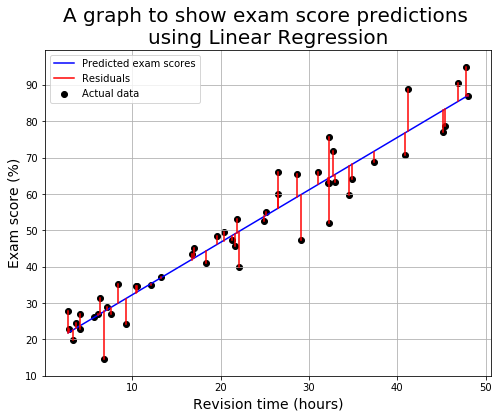
\includegraphics [width=1\textwidth]{images/q1b1.png}
\end{answerbox}



\end{subquestion}



%
%
\begin{subquestion}{(3 points) Instead of using sklearn, implement the closed-form solution for fitting a linear regression model yourself using numpy array operations.  
Report your code in the answer box.
It should only take a few lines (i.e. <5).\\ 
\hint{Only report the relevant lines for estimating $\mathbf{w}$ e.g. we do not need to see the data loading code. You can write the code in the answer box directly or paste in an image of it. }
}


\begin{answerbox}{24em}
\large{\textbf{\underline{Closed-form solution for fitting a linear regression model with}}}\\
\large{\textbf{\underline{numpy}}}\\
\\
\\
\normalsize{
\textbf{\underline{Given our analytical solution for calculating $\hat{\mathbf{w}}$:}}\\
\\
$\hat{\mathbf{w}} = (\mathbf{\Phi^{T}}\cdot\mathbf{\Phi})^{-1}\cdot\mathbf{\Phi^{T}}\cdot \mathbf{Y}$\\
\\
where $(\mathbf{\Phi^{T}}\cdot\mathbf{\Phi})^{-1}\cdot\mathbf{\Phi^{T}}$ is the pseudo-inverse of $\mathbf{\Phi}$
\\
\\
\\
\textbf{\underline{We can easily transfer this into code:}}\\
\\
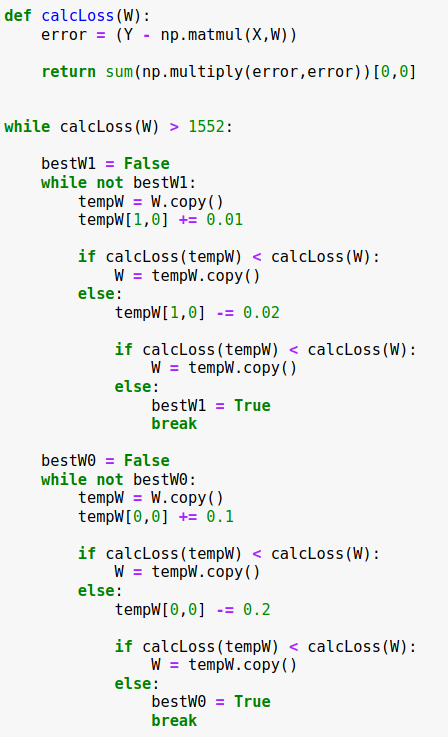
\includegraphics [width=1\textwidth]{images/q1d-code.png}
}
\end{answerbox}



\end{subquestion}



%
%
\begin{subquestion}{(3 points) Mean Squared Error (MSE) is a common metric used for evaluating the performance of regression models. 
Write out the expression for MSE and list one of its limitations. \\
\hint{For notation, you can use $y$ for the ground truth quantity and $\hat{y}$ (\texttt{\$\textbackslash{}hat\{y\}\$} in latex) in place of the model prediction.}
}


\begin{answerbox}{22em}
\large{\textbf{\underline{Limitations of the Mean Squared Error (MSE) metric}}}\\
\\
\normalsize{
$MSE = \sqrt{\frac{1}{n}\sum_{i=1}^{n}(\hat{y_i}-y_i)^2}$\\
\\
One of the disadvantages of the MSE metric is that it is very sensitive to outliers. This is evident in the equation as shown above, where for each value of x\textsubscript{i} the error value (difference in the predicted and actual value) of y\textsubscript{i} is squared and the average error value is calculated. This squaring of error values ultimately magnifies the large errors (caused by outliers) and minimizes the small errors. Inevitably meaning a single outlier in our dataset could skew our analysis greatly, due to the fact that we could get the same MSE for a predictor with one large error as a predictor with lots of small errors.\\
\\
The best way to solve such a problem would be through either identifying outliers in our dataset through visualization or using different error metrics which are more robust against outliers (eg. Median Absolute Deviation).}
\end{answerbox}



\end{subquestion}


 
%
%
\begin{subquestion}{(3 points) Our next step will be to evaluate the performance of the fitted models using Mean Squared Error (MSE). 
Report the MSE of the data in \texttt{regression\_part1.csv} for your prediction of \texttt{exam\_score}.
You should report the MSE for the linear model fitted using sklearn and the model resulting from your closed-form solution. 
Comment on any differences in their performance. 
}


\begin{answerbox}{20em}
\large{\textbf{\underline{Implementation evaluation using MSE}}}\\
\\
\\
\normalsize{
MSE\textsubscript{sklearn} = 30.985472614541305\\
%MAE = 4.246143979155163\\
%$R^{2}$ score = 0.9277934754398822\\
\\
MSE\textsubscript{closed-form} = 30.98547261454129\\
%MAE = 4.24614397915516\\
%$R^{2}$ score = 0.9277934754398822
\\
\\
\textbf{\underline{Differences in performance:}}\\
\\
$MSE\textsubscript{sklearn} = MSE\textsubscript{closed-form}   +   1.4210854715202004 * 10^{-14}$\\
\\
Given that both of these models were calculated on the exact same dataset, we can see that the solution of our closed-form implementation was a tiny bit more accurate than that of our sklearn implementation.
}
\end{answerbox}



\end{subquestion}




%
%
\begin{subquestion}{(4 points) Assume that the optimal value of $w_0$ is $20$, it is not but let's assume so for now. 
Create a plot where you vary $w_1$ from $-2$ to $+2$ on the horizontal axis, and report the Mean Squared Error on the vertical axis for each setting of $\mathbf{w} = [w_0, w_1]$ across the dataset. 
Describe the resulting plot. Where is its minimum? Is this value to be expected?\\ 
\hint{You can try 100 values of $w_1$ i.e. \texttt{w1 = np.linspace(-2,2, 100)}.}
}


\begin{answerbox}{48em}
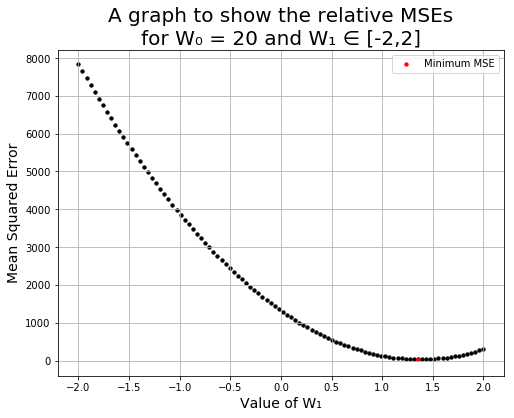
\includegraphics [width=1\textwidth]{images/q1g-graph.png}\\
\\
\\
This plot seems to take the form of a parabola, where the MSE increases exponentially either side of the global minimum MSE (illustrated by the red point). This shows just how important the decimal accuracy of our $\mathbf{w}$ value really is, as a small difference in this can result in a large difference in accuracy.\\
\\
$\mathbf{MSE_{min}} = 32.48096161535148$ ,  where $\mathbf{w_1} = 1.3535353535353538$\\
\\
This value of $\mathbf{w_1}$ is expected. We knew it had to be less than that of the optimum found in previous implementations (where $\mathbf{w_1} \approx 1.441$). This is due to the fact that we have set $\mathbf{w_0} = 20$, which is evidently greater than its optimum (where $\mathbf{w_0} \approx 17.898$).
\end{answerbox}



\end{subquestion}


 
\end{question}





%%%%%%%%%%%%%%%%%%%%%%%%%%%%%%%%%%%%%%%%%%%%%%%%%%%%%%%%%%%%%%%%%%%%%%%%%%%%%%
%============================================================================%
%%%%%%%%%%%%%%%%%%%%%%%%%%%%%%%%%%%%%%%%%%%%%%%%%%%%%%%%%%%%%%%%%%%%%%%%%%%%%%
\clearpage



\begin{question}{(18 total points) Nonlinear Regression}

\questiontext{In this question we will tackle regression using basis functions.}




%
%
\begin{subquestion}{(5 points) Fit four different polynomial regression models to the data  by varying the degree of polynomial features used i.e. $M = 1$ to $4$.
For example, $M=3$ means that $\boldsymbol{\phi}(x_i) = [1, x_i, x_i^2, x_i^3]$.
Plot the resulting models on the same plot and also include the input data.\\
\hint{
 You can again use the sklearn implementation of \href{https://scikit-learn.org/0.19/modules/generated/sklearn.linear_model.LinearRegression.html}{Linear Regression} and you can also use \href{https://scikit-learn.org/0.19/modules/generated/sklearn.preprocessing.PolynomialFeatures.html}{PolynomialFeatures} to generate the polynomial features. Again, set \texttt{fit\_intercept = False}.}
}


\begin{answerbox}{35em}
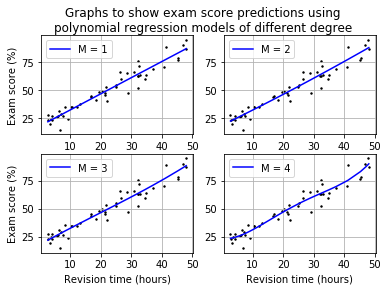
\includegraphics [width=1\textwidth]{images/q2a-graph.png}
\end{answerbox}



\end{subquestion}


%
%
\begin{subquestion}{(3 points) Create a bar plot where you display the Mean Squared Error of each of the four different polynomial regression models from the previous question.}


\begin{answerbox}{35em}
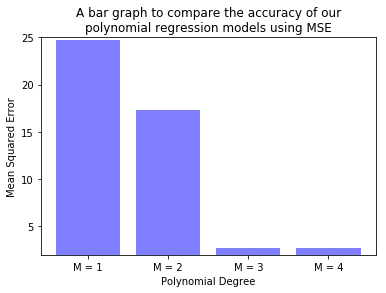
\includegraphics [width=1\textwidth]{images/q2b-graph.png}
\end{answerbox}



\end{subquestion}


%
%
\begin{subquestion}{(4 points) Comment on the fit and Mean Squared Error values of the $M=3$ and $M=4$ polynomial regression models. 
Do they result in the same or different performance? 
Based on these results, which model would you choose?}


\begin{answerbox}{23em}
\large{\textbf{\underline{Comparing the M=3 and M=4 polynomial regression models}}}\\
\\
\normalsize{
$MSE_{M=3} = 2.744756719252427$\\
$MSE_{M=4} = 2.738911179075539$\\
\\
Therefore:\\
$MSE_{M=3} = MSE_{M=4} + 0.005845540176887987$\\
\\
It is therefore evident that the M=4 model performs slightly better than the M=3 model on this given dataset. However we must be wary of overfitting these models to our training data. So before deciding on which model to use it would be useful to test and compare the performance of these models on a large unseen dataset.\\
\\
But since we are unable to test these models any further if I had to choose a model given it's MSE performance metric on this dataset alone I would choose the M=4 model.
}
\end{answerbox}



\end{subquestion}



%
%
\begin{subquestion}{(6 points) Instead of using polynomial basis functions, in this final part we will use another type of basis function - radial basis functions (RBF). 
Specifically, we will define $\boldsymbol{\phi}(x_i) = [1, rbf(x_i; c_1, \alpha), rbf(x_i; c_2, \alpha), rbf(x_i; c_3, \alpha), rbf(x_i; c_4, \alpha)]$, where $rbf(x; c, \alpha) =  \exp(-0.5(x-c)^2 / \alpha^2)$ is an RBF kernel with center $c$ and width $\alpha$. Note that in this example, we are using the same width $\alpha$ for each RBF, but different centers for each.\\ 
Let $c_1=-4.0$, $c_2=-2.0$, $c_3=2.0$, and $c_4=4.0$ and plot the resulting nonlinear predictions using the \texttt{regression\_part2.csv} dataset for $\alpha \in \{0.2, 100, 1000\}$. 
You can plot all three results on the same figure.
Comment on the impact of larger or smaller values of $\alpha$.
}


\begin{answerbox}{41em}
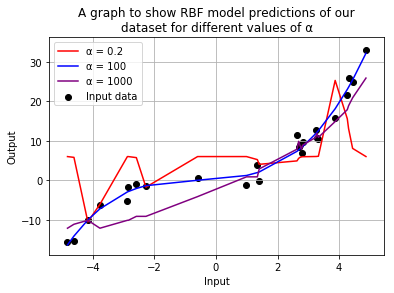
\includegraphics [width=1\textwidth]{images/q2d-graph.png}\\
\\
\textbf{\underline{Impact of $\mathbf{\alpha}$:}}\\
As illustrated on this figure it is evident that the RBF kernel with $\mathbf{\alpha} = 100$ creates the best classifier due to it's smooth model and close fit to all the data points.\\
\\
The RBF kernel with $\mathbf{\alpha} = 0.2$ seems to overfit the data in a dramatic way with a very "spikey" model that does not fit well to a large majority of the data points. In contrast, the RBF kernel with $\mathbf{\alpha} = 1000$ seems to underfit the data with a relatively straight model that does not fit well to a smaller majority of the data points.\\
\end{answerbox}



\end{subquestion}



\end{question}






%%%%%%%%%%%%%%%%%%%%%%%%%%%%%%%%%%%%%%%%%%%%%%%%%%%%%%%%%%%%%%%%%%%%%%%%%%%%%%
%============================================================================%
%%%%%%%%%%%%%%%%%%%%%%%%%%%%%%%%%%%%%%%%%%%%%%%%%%%%%%%%%%%%%%%%%%%%%%%%%%%%%%
\clearpage


\begin{question}{(26 total points) Decision Trees}

\questiontext{In this question we will train a classifier to predict if a person is smiling or not.}




%
%
\begin{subquestion}{(4 points) Load the data, taking care to separate the target binary class label we want to predict, \texttt{smiling}, from the input attributes. 
Summarise the main properties of both the training and test splits. 
}


\begin{answerbox}{30em}
\large{\textbf{\underline{INPUT DATA:}}}\\
\\
\fbox{
\parbox{30em}{
\normalsize{\textbf{\underline{Data properties of the 'faces\_train\_data.csv' dataset:}}}\\
\\
\footnotesize{
\textbf{Dataset size:} 4800 records\\
\textbf{Dataset shape:} (4800, 136)\\
\textbf{Data types:} all attribute values of type float64\\
}
\\
\\
\normalsize{\textbf{\underline{Data properties of the 'faces\_test\_data.csv' dataset:}}}\\
\\
\footnotesize{
\textbf{Dataset size:} 1200 records\\
\textbf{Dataset shape:} (1200, 136)\\
\textbf{Data types:} all attribute values of type float64\\
}
}}
\\
\\
\\
\large{\textbf{\underline{OUTPUT DATA:}}}\\
\\
\fbox{
\parbox{30em}{
\normalsize{\textbf{\underline{Data properties of "smiling" output attribute:}}}\\
\\
\footnotesize{
\textbf{Data type:} attribute value of type int64\\
\\
This "smiling" attribute is a binary value which is used to label whether a given piece of data represents someone smiling or not.
}
}}
\end{answerbox}



\end{subquestion}


%
%
\begin{subquestion}{(4 points) Even though the input attributes are high dimensional, they actually consist of a set of 2D coordinates representing points on the faces of each person in the dataset. 
Create a scatter plot of the average location for each 2D coordinate. One for (i) smiling and (ii) one not smiling faces. 
For instance, in the case of smiling faces, you would average each of the rows where \texttt{smiling = 1}. 
You can plot both on the same figure, but use different colors for each of the two cases. 
Comment on any difference you notice between the two sets of points. \\
\hint{Your plot should contain two faces.}
}


\begin{answerbox}{35em}
Your Answer Here
\end{answerbox}



\end{subquestion}


%
%
\begin{subquestion}{(2 points) 
There are different measures that can be used in decision trees when evaluating the quality of a split. 
What measure of purity at a node does the \href{https://scikit-learn.org/0.19/modules/generated/sklearn.tree.DecisionTreeClassifier.html}{DecisionTreeClassifier} in sklearn use for classification by default? 
What is the advantage, if any, of using this measure compared to entropy? 
}


\begin{answerbox}{10em}
Your Answer Here
\end{answerbox}



\end{subquestion}


%
%
\begin{subquestion}{(3 points) 
One of the hyper-parameters of a decision tree classifier is the maximum depth of the tree. 
What impact does smaller or larger values of this parameter have? Give one potential problem for small values and two for large values. 
}


\begin{answerbox}{10em}
Your Answer Here
\end{answerbox}



\end{subquestion}


%
%
\begin{subquestion}{(6 points) 
Train three different decision tree classifiers with a maximum depth of 2, 8, and 20 respectively.
Report the maximum depth, the training accuracy (in \%), and the test accuracy (in \%) for each of the three trees.
Comment on which model is best and why it is best. \\
\hint{Set \texttt{random\_state = 2001} and use the \texttt{predict()} method of the \href{https://scikit-learn.org/0.19/modules/generated/sklearn.tree.DecisionTreeClassifier.html}{DecisionTreeClassifier} so that you do not need to set a threshold on the output predictions.
You can set the maximum depth of the decision tree using the \texttt{max\_depth} hyper-parameter.}
}


\begin{answerbox}{20em}
Your Answer Here
\end{answerbox}



\end{subquestion}


%
%
\begin{subquestion}{(5 points) 
Report the names of the top three most important attributes, in order of importance, according to the Gini importance from \href{https://scikit-learn.org/0.19/modules/generated/sklearn.tree.DecisionTreeClassifier.html}{DecisionTreeClassifier}. 
Does the one with the highest importance make sense in the context of this classification task? \\
\hint{Use the trained model with \texttt{max\_depth = 8} and again set  \texttt{random\_state = 2001}.}
}


\begin{answerbox}{10em}
Your Answer Here
\end{answerbox}



\end{subquestion}



%
%
\begin{subquestion}{(2 points) 
Are there any limitations of the current choice of input attributes used i.e. 2D point locations? If so, name one. 
}


\begin{answerbox}{10em}
Your Answer Here
\end{answerbox}



\end{subquestion}


\end{question}




%%%%%%%%%%%%%%%%%%%%%%%%%%%%%%%%%%%%%%%%%%%%%%%%%%%%%%%%%%%%%%%%%%%%%%%%%%%%%%
%============================================================================%
%%%%%%%%%%%%%%%%%%%%%%%%%%%%%%%%%%%%%%%%%%%%%%%%%%%%%%%%%%%%%%%%%%%%%%%%%%%%%%
\clearpage


\begin{question}{(14 total points) Evaluating Binary Classifiers}

\questiontext{In this question we will perform performance evaluation of binary classifiers.}




%
%
\begin{subquestion}{(4 points) Report the classification accuracy (in \%) for each of the four different models using the \texttt{gt} attribute as the ground truth class labels. 
Use a threshold of $>= 0.5$ to convert the continuous classifier outputs into binary predictions. 
Which model is the best according to this metric?
What, if any, are the limitations of the above method for computing accuracy and how would you improve it without changing the metric used?
}


\begin{answerbox}{15em}
Your Answer Here
\end{answerbox}



\end{subquestion}



%
%
\begin{subquestion}{(4 points) Instead of using classification accuracy, report the Area Under the ROC Curve (AUC) for each model. 
Does the model with the best AUC also have the best accuracy? If not, why not?\\
\hint{You can use the  \href{https://scikit-learn.org/0.19/modules/generated/sklearn.metrics.roc\_auc\_score.html}{roc\_auc\_score} function from sklearn.}
}


\begin{answerbox}{15em}
Your Answer Here
\end{answerbox}



\end{subquestion}



%
%
\begin{subquestion}{(6 points) Plot ROC curves for each of the four models on the same plot.
Comment on the ROC curve for \texttt{alg\_3}?
Is there anything that can be done to improve the performance of \texttt{alg\_3} without having to retrain the model?\\
\hint{You can use the \href{https://scikit-learn.org/0.19/modules/generated/sklearn.metrics.roc\_curve.html}{roc\_curve} function from sklearn.}
}


\begin{answerbox}{35em}
Your Answer Here
\end{answerbox}



\end{subquestion}

\end{question}







\end{document}
